\section{Background}
\label{sec:background}

\paragraph{Docker image storage.} Docker~\cite{docker} is a containerization
platform to develop, deploy, and run applications inside \emph{containers}.
Users interact with Docker using the Docker client, which in turn sends
commands to the Docker host.  The Docker host runs a daemon process that
implements the core logic of Docker and is responsible for \emph{running}
containers from locally available images.  A Docker image consists of an
ordered series of \emph{layers}.  Each Docker layer contains a subset of the
files in the image and often represents a specific component/dependency of the
image, \eg a shared library.  Layers can be shared between two or more images
if the images depend on the same layer.  Image layers are read-only.  When
users start a container, Docker creates a new \emph{writable layer} on top of
the underlying read-only layers.
% (Figure~\ref{fig-docker-architecture}).
Any changes made to files in the image will be reflected inside the writable
layer via a copy-on-write~(COW) mechanism.

 %in a container image to simplify and automate application
 %deployment~\cite{slacker}.  for packaging, distributing, and running
 %applications.  The client can be co-located on the host machine. 
% 
%
 %If a user tries to launch a container from an image that is not available
 %locally, the daemon \texttt{pulls} the required image from the Docker registry.
 %Additionally, the daemon supports \texttt{building} new images and
 %\texttt{pushing} them to the registry.  


Docker registry~\cite{docker-hub} is a platform for storing and distributing container
images. It stores images in \emph{repositories}, each containing different
versions (\emph{tags}) of the same image, identified as
\texttt{<repo-name:tag>}.  For each image, the Docker registry stores a
\emph{manifest}.
The manifest is a JSON file, which contains the runtime configuration for a
container image (\eg target platform and environment variables) and the list
of layers which make up the image.
Layers are identified via a digest that is computed as a hash (SHA-256) over
the uncompressed content of the layer and stored as compressed archival files.
If a user tries to launch a container from an image that is not available
locally, it will \texttt{pulls} the required image from the Docker registry.
Additionally, the daemon supports \texttt{building} new images and
\texttt{pushing} them to the registry.  By using layer-level content
addressable store, Image layers are stored as compressed archival files and
image manifests as JSON files.

%
%Docker registry is a web server that serves docker pull and docker push
%requests.  

Although Docker registry
is a layer-level content addressable storage system storing all the images, it
delegates storage to drivers that interact with either a local file system or a
remote cloud storage such as Amazon S3~\cite{s3}, Microsoft Azure~\cite{azure},
OpenStack Swift~\cite{swift}, and Aliyun OSS~\cite{aliyun}.  For example,
Google Container Registry~\cite{GoogleContainerRegistry} uses Google cloud as
its backend image store.  Users \texttt{push} and \texttt{pull} Docker images
to and from their repositories that are stored on cloud storage. 
Upon a \texttt{push} layer request, Docker registry fowrards the layer to the
backend storage which stores multiple replicas of the layer.
The subsequent \texttt{pull} layer requests can be served by 
any of the three layer replicas.
Service providers often use geographically
distributed registries for faster access, e.g., IBM's Container Registry setup
spans five regions~\cite{dockerworkload}. 


%\Ali{Nannan: Please add a figure that show existing registry design}
%\LR{This following paragraph should be part of background. Ali, can you move it to background and fit
%it in there? I think we should also split Figure~\ref{fig:sift-original} and also move the top part,
%which describes the standard registry, to the background section.}


%

\begin{figure}
	\centering
	% Requires \usepackage{graphicx}
	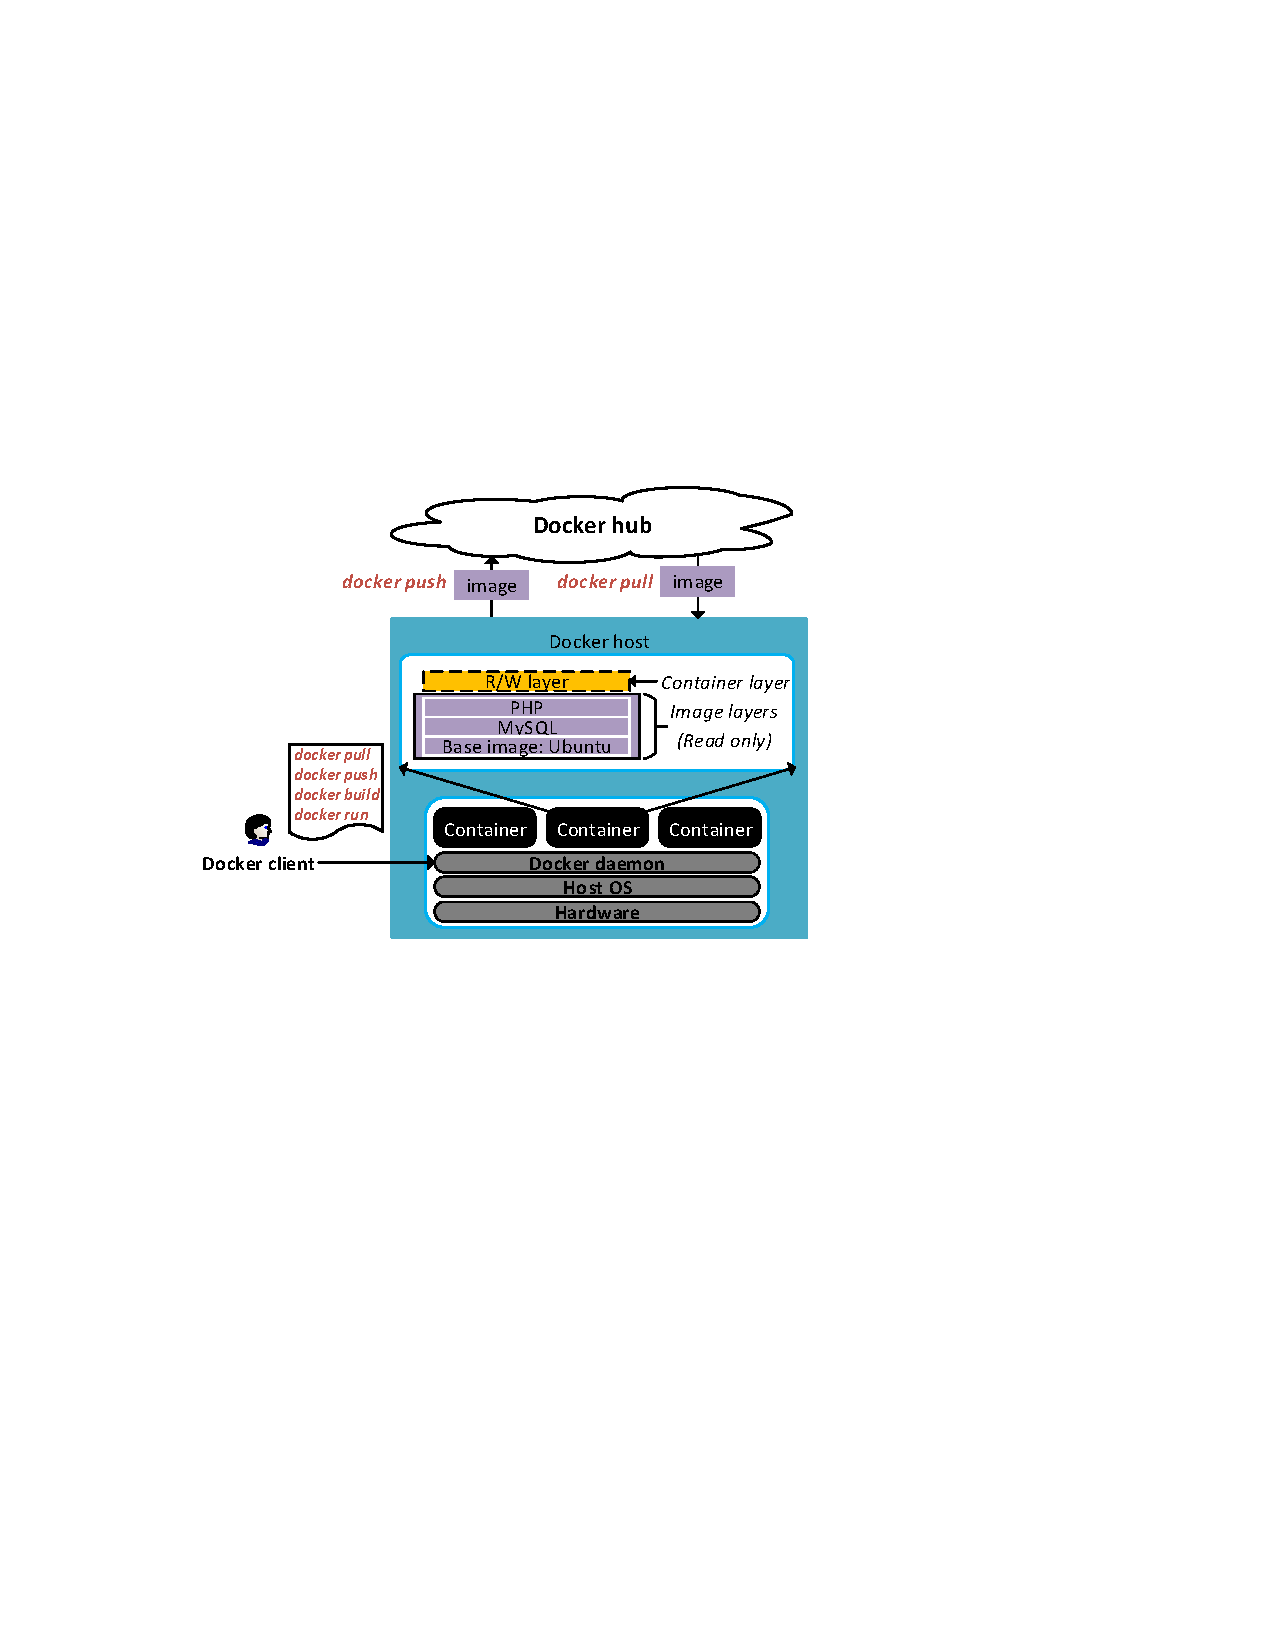
\includegraphics[width=0.5\textwidth]{graphs/fig-docker-architecture}
	\caption{Docker ecosystem
%	\lrcomment{We need to update the figure to capture
%	all the main interactions between the components and remove some unneeded
%	detail, \eg official and unofficial repositories\nancomment{addressed}}
	}
	\label{fig-docker-architecture}
\end{figure} As shown in
%Figure~\ref{fig-docker-architecture}, a typical Docker setup consists of three
%main components: \emph{client}, \emph{host}, and \emph{registry}.  
%Docker Hub
%is one of the most popular public registries, supporting both public and
%private repositories, via which users can upload, search, and download images.
%In Docker Hub, the user repositories are namespaced by user name, i.e.,
%``$\langle username\rangle/\langle repository name \rangle$", while the
%official repositories, which are directly provided by Docker Inc. and partners
%are called ``$\langle repository name \rangle$".   


\Ali{I am not sure how to weave in the following paragraph with the previous ones.}
\paragraph{Deduplication}
Most existing cloud storage
providers employ data deduplication techniques to eliminate redundant data,
same data stored more than once.  Deduplication techniques significantly reduce
storage needs and therefore reduce storage costs and improve storage
efficiency.  Data deduplication works by storing duplicate data chunks only
once, keeping only the unique data chunks. 
Current cloud providers deploy a
cross-user client-side fixed-size-chunk-level data deduplication that delivers
the highest deduplication gain~\cite{pooranian2018rare}.  These approaches
maximize the benefit of deduplication: The cross-user data deduplication treats
cloud storage as a pool shared by all the cloud users, because the potential
for data deduplication is the highest as the probability for redundancies and
duplicates is higher the more inclusive the shared pool.  The
fixed-size-chunk-level specifies that a fixed-size chunk is the unit for
checking for duplicates on cloud storage.  Google cloud and AWS employ
StorReduce, a deduplication software that performs in-line data deduplication
transparently and resides between the client's application and the hosting
cloud storage. StorReduce provide 80-97\% storage and bandwidth reduction to
the cloud providers~\cite{StorReduce_google}.  
%server-side data deduplication?


